\documentclass[12pt]{article}

\usepackage{amsmath, amssymb}
\usepackage[margin=1in]{geometry}
\usepackage{helvet}
\renewcommand{\familydefault}{\sfdefault}
\def\newrule#1#2#3{\begin{center}
    {#1} \\
    \line(1,0){300} {}{}{}{}{}{}{} [{#3}]\\
    {#2}
\end{center}}

\begin{document}
\def\assignment{Homework 08}

\pagenumbering{gobble}
\noindent{\large COSC 4765 \hfill Name: \underline{Jacob Tuttle} \\ Computer Security}
\begin{center}
    {\Large \assignment} \\ \textbf{\today}
\end{center}
\vspace{5mm}

\question{A depiction of the System}

% system drawing, collapsed to save space
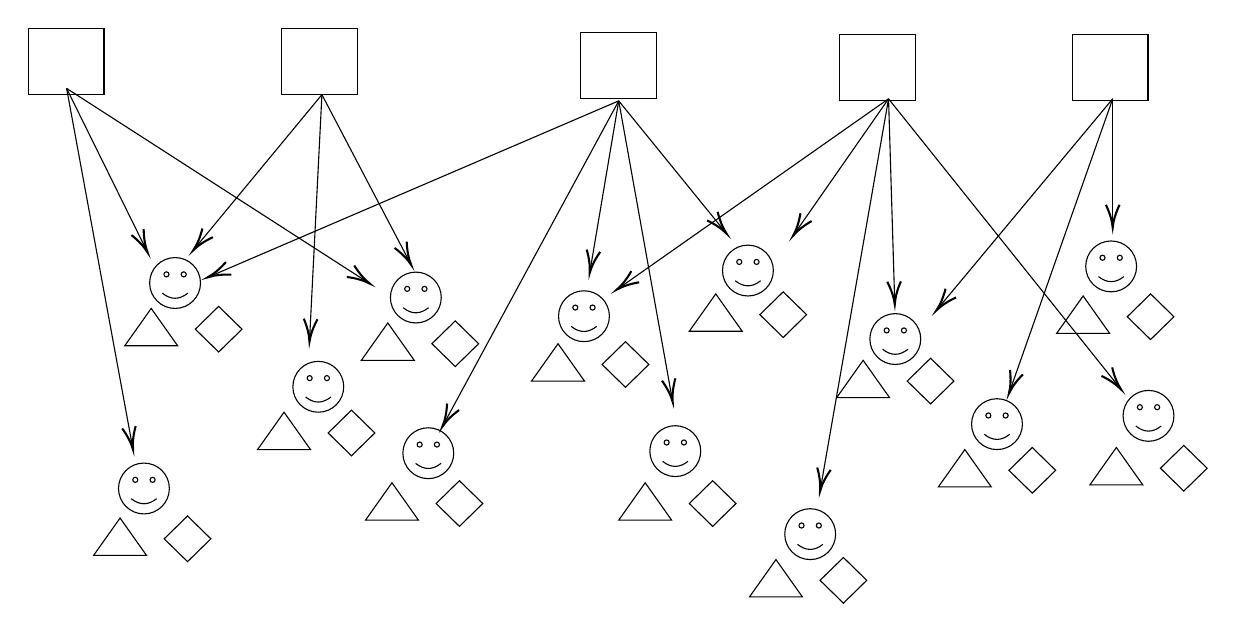
\begin{tikzpicture}[x=0.75pt,y=0.75pt,yscale=-1,xscale=1]
%uncomment if require: \path (0,300); %set diagram left start at 0, and has height of 300

%Shape: Rectangle [id:dp6309471025073041] 
\draw   (33,13) -- (69.5,13) -- (69.5,45) -- (33,45) -- cycle ;
%Shape: Rectangle [id:dp14560251331380725] 
\draw   (155,13) -- (191.5,13) -- (191.5,45) -- (155,45) -- cycle ;
%Shape: Rectangle [id:dp634612683436614] 
\draw   (299,15) -- (335.5,15) -- (335.5,47) -- (299,47) -- cycle ;
%Shape: Rectangle [id:dp4682674793582309] 
\draw   (424,16) -- (460.5,16) -- (460.5,48) -- (424,48) -- cycle ;
%Shape: Rectangle [id:dp9514025305157071] 
\draw   (536,16) -- (572.5,16) -- (572.5,48) -- (536,48) -- cycle ;
%Shape: Smiley Face [id:dp4179402090500539] 
\draw   (91.5,135.75) .. controls (91.5,128.98) and (96.98,123.5) .. (103.75,123.5) .. controls (110.52,123.5) and (116,128.98) .. (116,135.75) .. controls (116,142.52) and (110.52,148) .. (103.75,148) .. controls (96.98,148) and (91.5,142.52) .. (91.5,135.75) -- cycle ; \draw   (98.36,131.59) .. controls (98.36,130.91) and (98.91,130.36) .. (99.59,130.36) .. controls (100.26,130.36) and (100.81,130.91) .. (100.81,131.59) .. controls (100.81,132.26) and (100.26,132.81) .. (99.59,132.81) .. controls (98.91,132.81) and (98.36,132.26) .. (98.36,131.59) -- cycle ; \draw   (106.69,131.59) .. controls (106.69,130.91) and (107.24,130.36) .. (107.92,130.36) .. controls (108.59,130.36) and (109.14,130.91) .. (109.14,131.59) .. controls (109.14,132.26) and (108.59,132.81) .. (107.92,132.81) .. controls (107.24,132.81) and (106.69,132.26) .. (106.69,131.59) -- cycle ; \draw   (97.63,140.65) .. controls (101.71,143.92) and (105.79,143.92) .. (109.88,140.65) ;
%Shape: Smiley Face [id:dp9412585591825343] 
\draw   (207.5,142.75) .. controls (207.5,135.98) and (212.98,130.5) .. (219.75,130.5) .. controls (226.52,130.5) and (232,135.98) .. (232,142.75) .. controls (232,149.52) and (226.52,155) .. (219.75,155) .. controls (212.98,155) and (207.5,149.52) .. (207.5,142.75) -- cycle ; \draw   (214.36,138.59) .. controls (214.36,137.91) and (214.91,137.36) .. (215.59,137.36) .. controls (216.26,137.36) and (216.81,137.91) .. (216.81,138.59) .. controls (216.81,139.26) and (216.26,139.81) .. (215.59,139.81) .. controls (214.91,139.81) and (214.36,139.26) .. (214.36,138.59) -- cycle ; \draw   (222.69,138.59) .. controls (222.69,137.91) and (223.24,137.36) .. (223.92,137.36) .. controls (224.59,137.36) and (225.14,137.91) .. (225.14,138.59) .. controls (225.14,139.26) and (224.59,139.81) .. (223.92,139.81) .. controls (223.24,139.81) and (222.69,139.26) .. (222.69,138.59) -- cycle ; \draw   (213.63,147.65) .. controls (217.71,150.92) and (221.79,150.92) .. (225.88,147.65) ;
%Shape: Smiley Face [id:dp7967400793331137] 
\draw   (560.5,199.75) .. controls (560.5,192.98) and (565.98,187.5) .. (572.75,187.5) .. controls (579.52,187.5) and (585,192.98) .. (585,199.75) .. controls (585,206.52) and (579.52,212) .. (572.75,212) .. controls (565.98,212) and (560.5,206.52) .. (560.5,199.75) -- cycle ; \draw   (567.36,195.59) .. controls (567.36,194.91) and (567.91,194.36) .. (568.59,194.36) .. controls (569.26,194.36) and (569.81,194.91) .. (569.81,195.59) .. controls (569.81,196.26) and (569.26,196.81) .. (568.59,196.81) .. controls (567.91,196.81) and (567.36,196.26) .. (567.36,195.59) -- cycle ; \draw   (575.69,195.59) .. controls (575.69,194.91) and (576.24,194.36) .. (576.92,194.36) .. controls (577.59,194.36) and (578.14,194.91) .. (578.14,195.59) .. controls (578.14,196.26) and (577.59,196.81) .. (576.92,196.81) .. controls (576.24,196.81) and (575.69,196.26) .. (575.69,195.59) -- cycle ; \draw   (566.63,204.65) .. controls (570.71,207.92) and (574.79,207.92) .. (578.88,204.65) ;
%Shape: Smiley Face [id:dp806959687924422] 
\draw   (487.5,203.75) .. controls (487.5,196.98) and (492.98,191.5) .. (499.75,191.5) .. controls (506.52,191.5) and (512,196.98) .. (512,203.75) .. controls (512,210.52) and (506.52,216) .. (499.75,216) .. controls (492.98,216) and (487.5,210.52) .. (487.5,203.75) -- cycle ; \draw   (494.36,199.59) .. controls (494.36,198.91) and (494.91,198.36) .. (495.59,198.36) .. controls (496.26,198.36) and (496.81,198.91) .. (496.81,199.59) .. controls (496.81,200.26) and (496.26,200.81) .. (495.59,200.81) .. controls (494.91,200.81) and (494.36,200.26) .. (494.36,199.59) -- cycle ; \draw   (502.69,199.59) .. controls (502.69,198.91) and (503.24,198.36) .. (503.92,198.36) .. controls (504.59,198.36) and (505.14,198.91) .. (505.14,199.59) .. controls (505.14,200.26) and (504.59,200.81) .. (503.92,200.81) .. controls (503.24,200.81) and (502.69,200.26) .. (502.69,199.59) -- cycle ; \draw   (493.63,208.65) .. controls (497.71,211.92) and (501.79,211.92) .. (505.88,208.65) ;
%Shape: Smiley Face [id:dp32176010424299395] 
\draw   (542.5,127.75) .. controls (542.5,120.98) and (547.98,115.5) .. (554.75,115.5) .. controls (561.52,115.5) and (567,120.98) .. (567,127.75) .. controls (567,134.52) and (561.52,140) .. (554.75,140) .. controls (547.98,140) and (542.5,134.52) .. (542.5,127.75) -- cycle ; \draw   (549.36,123.59) .. controls (549.36,122.91) and (549.91,122.36) .. (550.59,122.36) .. controls (551.26,122.36) and (551.81,122.91) .. (551.81,123.59) .. controls (551.81,124.26) and (551.26,124.81) .. (550.59,124.81) .. controls (549.91,124.81) and (549.36,124.26) .. (549.36,123.59) -- cycle ; \draw   (557.69,123.59) .. controls (557.69,122.91) and (558.24,122.36) .. (558.92,122.36) .. controls (559.59,122.36) and (560.14,122.91) .. (560.14,123.59) .. controls (560.14,124.26) and (559.59,124.81) .. (558.92,124.81) .. controls (558.24,124.81) and (557.69,124.26) .. (557.69,123.59) -- cycle ; \draw   (548.63,132.65) .. controls (552.71,135.92) and (556.79,135.92) .. (560.88,132.65) ;
%Shape: Smiley Face [id:dp29273986019093] 
\draw   (397.5,256.75) .. controls (397.5,249.98) and (402.98,244.5) .. (409.75,244.5) .. controls (416.52,244.5) and (422,249.98) .. (422,256.75) .. controls (422,263.52) and (416.52,269) .. (409.75,269) .. controls (402.98,269) and (397.5,263.52) .. (397.5,256.75) -- cycle ; \draw   (404.36,252.59) .. controls (404.36,251.91) and (404.91,251.36) .. (405.59,251.36) .. controls (406.26,251.36) and (406.81,251.91) .. (406.81,252.59) .. controls (406.81,253.26) and (406.26,253.81) .. (405.59,253.81) .. controls (404.91,253.81) and (404.36,253.26) .. (404.36,252.59) -- cycle ; \draw   (412.69,252.59) .. controls (412.69,251.91) and (413.24,251.36) .. (413.92,251.36) .. controls (414.59,251.36) and (415.14,251.91) .. (415.14,252.59) .. controls (415.14,253.26) and (414.59,253.81) .. (413.92,253.81) .. controls (413.24,253.81) and (412.69,253.26) .. (412.69,252.59) -- cycle ; \draw   (403.63,261.65) .. controls (407.71,264.92) and (411.79,264.92) .. (415.88,261.65) ;
%Shape: Smiley Face [id:dp5194611398856444] 
\draw   (438.5,162.75) .. controls (438.5,155.98) and (443.98,150.5) .. (450.75,150.5) .. controls (457.52,150.5) and (463,155.98) .. (463,162.75) .. controls (463,169.52) and (457.52,175) .. (450.75,175) .. controls (443.98,175) and (438.5,169.52) .. (438.5,162.75) -- cycle ; \draw   (445.36,158.59) .. controls (445.36,157.91) and (445.91,157.36) .. (446.59,157.36) .. controls (447.26,157.36) and (447.81,157.91) .. (447.81,158.59) .. controls (447.81,159.26) and (447.26,159.81) .. (446.59,159.81) .. controls (445.91,159.81) and (445.36,159.26) .. (445.36,158.59) -- cycle ; \draw   (453.69,158.59) .. controls (453.69,157.91) and (454.24,157.36) .. (454.92,157.36) .. controls (455.59,157.36) and (456.14,157.91) .. (456.14,158.59) .. controls (456.14,159.26) and (455.59,159.81) .. (454.92,159.81) .. controls (454.24,159.81) and (453.69,159.26) .. (453.69,158.59) -- cycle ; \draw   (444.63,167.65) .. controls (448.71,170.92) and (452.79,170.92) .. (456.88,167.65) ;
%Shape: Smiley Face [id:dp7949474538069375] 
\draw   (332.5,216.75) .. controls (332.5,209.98) and (337.98,204.5) .. (344.75,204.5) .. controls (351.52,204.5) and (357,209.98) .. (357,216.75) .. controls (357,223.52) and (351.52,229) .. (344.75,229) .. controls (337.98,229) and (332.5,223.52) .. (332.5,216.75) -- cycle ; \draw   (339.36,212.59) .. controls (339.36,211.91) and (339.91,211.36) .. (340.59,211.36) .. controls (341.26,211.36) and (341.81,211.91) .. (341.81,212.59) .. controls (341.81,213.26) and (341.26,213.81) .. (340.59,213.81) .. controls (339.91,213.81) and (339.36,213.26) .. (339.36,212.59) -- cycle ; \draw   (347.69,212.59) .. controls (347.69,211.91) and (348.24,211.36) .. (348.92,211.36) .. controls (349.59,211.36) and (350.14,211.91) .. (350.14,212.59) .. controls (350.14,213.26) and (349.59,213.81) .. (348.92,213.81) .. controls (348.24,213.81) and (347.69,213.26) .. (347.69,212.59) -- cycle ; \draw   (338.63,221.65) .. controls (342.71,224.92) and (346.79,224.92) .. (350.88,221.65) ;
%Shape: Smiley Face [id:dp3733176540032682] 
\draw   (367.5,129.75) .. controls (367.5,122.98) and (372.98,117.5) .. (379.75,117.5) .. controls (386.52,117.5) and (392,122.98) .. (392,129.75) .. controls (392,136.52) and (386.52,142) .. (379.75,142) .. controls (372.98,142) and (367.5,136.52) .. (367.5,129.75) -- cycle ; \draw   (374.36,125.59) .. controls (374.36,124.91) and (374.91,124.36) .. (375.59,124.36) .. controls (376.26,124.36) and (376.81,124.91) .. (376.81,125.59) .. controls (376.81,126.26) and (376.26,126.81) .. (375.59,126.81) .. controls (374.91,126.81) and (374.36,126.26) .. (374.36,125.59) -- cycle ; \draw   (382.69,125.59) .. controls (382.69,124.91) and (383.24,124.36) .. (383.92,124.36) .. controls (384.59,124.36) and (385.14,124.91) .. (385.14,125.59) .. controls (385.14,126.26) and (384.59,126.81) .. (383.92,126.81) .. controls (383.24,126.81) and (382.69,126.26) .. (382.69,125.59) -- cycle ; \draw   (373.63,134.65) .. controls (377.71,137.92) and (381.79,137.92) .. (385.88,134.65) ;
%Shape: Smiley Face [id:dp9107544165626518] 
\draw   (76.5,234.75) .. controls (76.5,227.98) and (81.98,222.5) .. (88.75,222.5) .. controls (95.52,222.5) and (101,227.98) .. (101,234.75) .. controls (101,241.52) and (95.52,247) .. (88.75,247) .. controls (81.98,247) and (76.5,241.52) .. (76.5,234.75) -- cycle ; \draw   (83.36,230.59) .. controls (83.36,229.91) and (83.91,229.36) .. (84.59,229.36) .. controls (85.26,229.36) and (85.81,229.91) .. (85.81,230.59) .. controls (85.81,231.26) and (85.26,231.81) .. (84.59,231.81) .. controls (83.91,231.81) and (83.36,231.26) .. (83.36,230.59) -- cycle ; \draw   (91.69,230.59) .. controls (91.69,229.91) and (92.24,229.36) .. (92.92,229.36) .. controls (93.59,229.36) and (94.14,229.91) .. (94.14,230.59) .. controls (94.14,231.26) and (93.59,231.81) .. (92.92,231.81) .. controls (92.24,231.81) and (91.69,231.26) .. (91.69,230.59) -- cycle ; \draw   (82.63,239.65) .. controls (86.71,242.92) and (90.79,242.92) .. (94.88,239.65) ;
%Shape: Smiley Face [id:dp3589931760897165] 
\draw   (213.5,217.75) .. controls (213.5,210.98) and (218.98,205.5) .. (225.75,205.5) .. controls (232.52,205.5) and (238,210.98) .. (238,217.75) .. controls (238,224.52) and (232.52,230) .. (225.75,230) .. controls (218.98,230) and (213.5,224.52) .. (213.5,217.75) -- cycle ; \draw   (220.36,213.59) .. controls (220.36,212.91) and (220.91,212.36) .. (221.59,212.36) .. controls (222.26,212.36) and (222.81,212.91) .. (222.81,213.59) .. controls (222.81,214.26) and (222.26,214.81) .. (221.59,214.81) .. controls (220.91,214.81) and (220.36,214.26) .. (220.36,213.59) -- cycle ; \draw   (228.69,213.59) .. controls (228.69,212.91) and (229.24,212.36) .. (229.92,212.36) .. controls (230.59,212.36) and (231.14,212.91) .. (231.14,213.59) .. controls (231.14,214.26) and (230.59,214.81) .. (229.92,214.81) .. controls (229.24,214.81) and (228.69,214.26) .. (228.69,213.59) -- cycle ; \draw   (219.63,222.65) .. controls (223.71,225.92) and (227.79,225.92) .. (231.88,222.65) ;
%Shape: Smiley Face [id:dp5543856329125892] 
\draw   (288.5,151.75) .. controls (288.5,144.98) and (293.98,139.5) .. (300.75,139.5) .. controls (307.52,139.5) and (313,144.98) .. (313,151.75) .. controls (313,158.52) and (307.52,164) .. (300.75,164) .. controls (293.98,164) and (288.5,158.52) .. (288.5,151.75) -- cycle ; \draw   (295.36,147.59) .. controls (295.36,146.91) and (295.91,146.36) .. (296.58,146.36) .. controls (297.26,146.36) and (297.81,146.91) .. (297.81,147.59) .. controls (297.81,148.26) and (297.26,148.81) .. (296.58,148.81) .. controls (295.91,148.81) and (295.36,148.26) .. (295.36,147.59) -- cycle ; \draw   (303.69,147.59) .. controls (303.69,146.91) and (304.24,146.36) .. (304.92,146.36) .. controls (305.59,146.36) and (306.14,146.91) .. (306.14,147.59) .. controls (306.14,148.26) and (305.59,148.81) .. (304.92,148.81) .. controls (304.24,148.81) and (303.69,148.26) .. (303.69,147.59) -- cycle ; \draw   (294.63,156.65) .. controls (298.71,159.92) and (302.79,159.92) .. (306.88,156.65) ;
%Shape: Smiley Face [id:dp3233193349478942] 
\draw   (160.5,185.75) .. controls (160.5,178.98) and (165.98,173.5) .. (172.75,173.5) .. controls (179.52,173.5) and (185,178.98) .. (185,185.75) .. controls (185,192.52) and (179.52,198) .. (172.75,198) .. controls (165.98,198) and (160.5,192.52) .. (160.5,185.75) -- cycle ; \draw   (167.36,181.59) .. controls (167.36,180.91) and (167.91,180.36) .. (168.59,180.36) .. controls (169.26,180.36) and (169.81,180.91) .. (169.81,181.59) .. controls (169.81,182.26) and (169.26,182.81) .. (168.59,182.81) .. controls (167.91,182.81) and (167.36,182.26) .. (167.36,181.59) -- cycle ; \draw   (175.69,181.59) .. controls (175.69,180.91) and (176.24,180.36) .. (176.92,180.36) .. controls (177.59,180.36) and (178.14,180.91) .. (178.14,181.59) .. controls (178.14,182.26) and (177.59,182.81) .. (176.92,182.81) .. controls (176.24,182.81) and (175.69,182.26) .. (175.69,181.59) -- cycle ; \draw   (166.63,190.65) .. controls (170.71,193.92) and (174.79,193.92) .. (178.88,190.65) ;
%Straight Lines [id:da8802909109040027] 
\draw    (51.5,42) -- (89.61,119.21) ;
\draw [shift={(90.5,121)}, rotate = 243.73] [color={rgb, 255:red, 0; green, 0; blue, 0 }  ][line width=0.75]    (10.93,-3.29) .. controls (6.95,-1.4) and (3.31,-0.3) .. (0,0) .. controls (3.31,0.3) and (6.95,1.4) .. (10.93,3.29)   ;
%Straight Lines [id:da8986682712209907] 
\draw    (51.5,42) -- (195.82,134.92) ;
\draw [shift={(197.5,136)}, rotate = 212.77] [color={rgb, 255:red, 0; green, 0; blue, 0 }  ][line width=0.75]    (10.93,-3.29) .. controls (6.95,-1.4) and (3.31,-0.3) .. (0,0) .. controls (3.31,0.3) and (6.95,1.4) .. (10.93,3.29)   ;
%Straight Lines [id:da3132644855262986] 
\draw    (51.5,42) -- (83.14,214.03) ;
\draw [shift={(83.5,216)}, rotate = 259.58] [color={rgb, 255:red, 0; green, 0; blue, 0 }  ][line width=0.75]    (10.93,-3.29) .. controls (6.95,-1.4) and (3.31,-0.3) .. (0,0) .. controls (3.31,0.3) and (6.95,1.4) .. (10.93,3.29)   ;
%Straight Lines [id:da6048025013121956] 
\draw    (174.5,45) -- (113.77,118.46) ;
\draw [shift={(112.5,120)}, rotate = 309.58000000000004] [color={rgb, 255:red, 0; green, 0; blue, 0 }  ][line width=0.75]    (10.93,-3.29) .. controls (6.95,-1.4) and (3.31,-0.3) .. (0,0) .. controls (3.31,0.3) and (6.95,1.4) .. (10.93,3.29)   ;
%Straight Lines [id:da9742488869374053] 
\draw    (174.5,45) -- (216.57,125.23) ;
\draw [shift={(217.5,127)}, rotate = 242.32999999999998] [color={rgb, 255:red, 0; green, 0; blue, 0 }  ][line width=0.75]    (10.93,-3.29) .. controls (6.95,-1.4) and (3.31,-0.3) .. (0,0) .. controls (3.31,0.3) and (6.95,1.4) .. (10.93,3.29)   ;
%Straight Lines [id:da2982557890774806] 
\draw    (174.5,45) -- (168.6,162) ;
\draw [shift={(168.5,164)}, rotate = 272.89] [color={rgb, 255:red, 0; green, 0; blue, 0 }  ][line width=0.75]    (10.93,-3.29) .. controls (6.95,-1.4) and (3.31,-0.3) .. (0,0) .. controls (3.31,0.3) and (6.95,1.4) .. (10.93,3.29)   ;
%Straight Lines [id:da8751001560857544] 
\draw    (317.5,48) -- (233.45,203.24) ;
\draw [shift={(232.5,205)}, rotate = 298.43] [color={rgb, 255:red, 0; green, 0; blue, 0 }  ][line width=0.75]    (10.93,-3.29) .. controls (6.95,-1.4) and (3.31,-0.3) .. (0,0) .. controls (3.31,0.3) and (6.95,1.4) .. (10.93,3.29)   ;
%Straight Lines [id:da36467153919933615] 
\draw    (317.5,48) -- (303.83,129.03) ;
\draw [shift={(303.5,131)}, rotate = 279.57] [color={rgb, 255:red, 0; green, 0; blue, 0 }  ][line width=0.75]    (10.93,-3.29) .. controls (6.95,-1.4) and (3.31,-0.3) .. (0,0) .. controls (3.31,0.3) and (6.95,1.4) .. (10.93,3.29)   ;
%Straight Lines [id:da5559513579262092] 
\draw    (317.5,48) -- (121.34,132.21) ;
\draw [shift={(119.5,133)}, rotate = 336.77] [color={rgb, 255:red, 0; green, 0; blue, 0 }  ][line width=0.75]    (10.93,-3.29) .. controls (6.95,-1.4) and (3.31,-0.3) .. (0,0) .. controls (3.31,0.3) and (6.95,1.4) .. (10.93,3.29)   ;
%Straight Lines [id:da6697069675705585] 
\draw    (317.5,48) -- (343.15,191.03) ;
\draw [shift={(343.5,193)}, rotate = 259.83] [color={rgb, 255:red, 0; green, 0; blue, 0 }  ][line width=0.75]    (10.93,-3.29) .. controls (6.95,-1.4) and (3.31,-0.3) .. (0,0) .. controls (3.31,0.3) and (6.95,1.4) .. (10.93,3.29)   ;
%Straight Lines [id:da7387223340829897] 
\draw    (317.5,48) -- (368.24,110.45) ;
\draw [shift={(369.5,112)}, rotate = 230.91] [color={rgb, 255:red, 0; green, 0; blue, 0 }  ][line width=0.75]    (10.93,-3.29) .. controls (6.95,-1.4) and (3.31,-0.3) .. (0,0) .. controls (3.31,0.3) and (6.95,1.4) .. (10.93,3.29)   ;
%Straight Lines [id:da49918411266052476] 
\draw    (447.5,47) -- (318.14,137.85) ;
\draw [shift={(316.5,139)}, rotate = 324.91999999999996] [color={rgb, 255:red, 0; green, 0; blue, 0 }  ][line width=0.75]    (10.93,-3.29) .. controls (6.95,-1.4) and (3.31,-0.3) .. (0,0) .. controls (3.31,0.3) and (6.95,1.4) .. (10.93,3.29)   ;
%Straight Lines [id:da6469559377178983] 
\draw    (447.5,47) -- (414.84,234.03) ;
\draw [shift={(414.5,236)}, rotate = 279.9] [color={rgb, 255:red, 0; green, 0; blue, 0 }  ][line width=0.75]    (10.93,-3.29) .. controls (6.95,-1.4) and (3.31,-0.3) .. (0,0) .. controls (3.31,0.3) and (6.95,1.4) .. (10.93,3.29)   ;
%Straight Lines [id:da05857800069587216] 
\draw    (447.5,47) -- (450.44,144) ;
\draw [shift={(450.5,146)}, rotate = 268.26] [color={rgb, 255:red, 0; green, 0; blue, 0 }  ][line width=0.75]    (10.93,-3.29) .. controls (6.95,-1.4) and (3.31,-0.3) .. (0,0) .. controls (3.31,0.3) and (6.95,1.4) .. (10.93,3.29)   ;
%Straight Lines [id:da6355107143086778] 
\draw    (447.5,47) -- (402.64,111.36) ;
\draw [shift={(401.5,113)}, rotate = 304.88] [color={rgb, 255:red, 0; green, 0; blue, 0 }  ][line width=0.75]    (10.93,-3.29) .. controls (6.95,-1.4) and (3.31,-0.3) .. (0,0) .. controls (3.31,0.3) and (6.95,1.4) .. (10.93,3.29)   ;
%Straight Lines [id:da2942335596468527] 
\draw    (447.5,47) -- (558.25,185.44) ;
\draw [shift={(559.5,187)}, rotate = 231.34] [color={rgb, 255:red, 0; green, 0; blue, 0 }  ][line width=0.75]    (10.93,-3.29) .. controls (6.95,-1.4) and (3.31,-0.3) .. (0,0) .. controls (3.31,0.3) and (6.95,1.4) .. (10.93,3.29)   ;
%Straight Lines [id:da49413860897012196] 
\draw    (555.5,47) -- (555.5,107) ;
\draw [shift={(555.5,109)}, rotate = 270] [color={rgb, 255:red, 0; green, 0; blue, 0 }  ][line width=0.75]    (10.93,-3.29) .. controls (6.95,-1.4) and (3.31,-0.3) .. (0,0) .. controls (3.31,0.3) and (6.95,1.4) .. (10.93,3.29)   ;
%Straight Lines [id:da8394975081082416] 
\draw    (555.5,47) -- (506.16,187.11) ;
\draw [shift={(505.5,189)}, rotate = 289.4] [color={rgb, 255:red, 0; green, 0; blue, 0 }  ][line width=0.75]    (10.93,-3.29) .. controls (6.95,-1.4) and (3.31,-0.3) .. (0,0) .. controls (3.31,0.3) and (6.95,1.4) .. (10.93,3.29)   ;
%Straight Lines [id:da29746772920466513] 
\draw    (555.5,47) -- (471.78,147.46) ;
\draw [shift={(470.5,149)}, rotate = 309.81] [color={rgb, 255:red, 0; green, 0; blue, 0 }  ][line width=0.75]    (10.93,-3.29) .. controls (6.95,-1.4) and (3.31,-0.3) .. (0,0) .. controls (3.31,0.3) and (6.95,1.4) .. (10.93,3.29)   ;
%Shape: Triangle [id:dp829092827643681] 
\draw   (92.25,148) -- (105,166) -- (79.5,166) -- cycle ;
%Shape: Diamond [id:dp3344714426618335] 
\draw   (124.75,147) -- (136,158) -- (124.75,169) -- (113.5,158) -- cycle ;
%Shape: Triangle [id:dp9831824608735396] 
\draw   (77.25,249) -- (90,267) -- (64.5,267) -- cycle ;
%Shape: Diamond [id:dp5730171745052058] 
\draw   (109.75,248) -- (121,259) -- (109.75,270) -- (98.5,259) -- cycle ;
%Shape: Triangle [id:dp04231340909462866] 
\draw   (156.25,198) -- (169,216) -- (143.5,216) -- cycle ;
%Shape: Diamond [id:dp387396878565502] 
\draw   (188.75,197) -- (200,208) -- (188.75,219) -- (177.5,208) -- cycle ;
%Shape: Triangle [id:dp8731440454142075] 
\draw   (206.25,155) -- (219,173) -- (193.5,173) -- cycle ;
%Shape: Diamond [id:dp6410207308305239] 
\draw   (238.75,154) -- (250,165) -- (238.75,176) -- (227.5,165) -- cycle ;
%Shape: Triangle [id:dp24716390731341942] 
\draw   (208.25,232) -- (221,250) -- (195.5,250) -- cycle ;
%Shape: Diamond [id:dp22003268628466977] 
\draw   (240.75,231) -- (252,242) -- (240.75,253) -- (229.5,242) -- cycle ;
%Shape: Triangle [id:dp6233550993837412] 
\draw   (288.25,165) -- (301,183) -- (275.5,183) -- cycle ;
%Shape: Diamond [id:dp34191547889647544] 
\draw   (320.75,164) -- (332,175) -- (320.75,186) -- (309.5,175) -- cycle ;
%Shape: Triangle [id:dp3213328608669779] 
\draw   (364.25,141) -- (377,159) -- (351.5,159) -- cycle ;
%Shape: Diamond [id:dp9556550552434964] 
\draw   (396.75,140) -- (408,151) -- (396.75,162) -- (385.5,151) -- cycle ;
%Shape: Triangle [id:dp502789642671312] 
\draw   (330.25,232) -- (343,250) -- (317.5,250) -- cycle ;
%Shape: Diamond [id:dp6702744209468625] 
\draw   (362.75,231) -- (374,242) -- (362.75,253) -- (351.5,242) -- cycle ;
%Shape: Triangle [id:dp20939172566435427] 
\draw   (435.25,173) -- (448,191) -- (422.5,191) -- cycle ;
%Shape: Diamond [id:dp08546575287590319] 
\draw   (467.75,172) -- (479,183) -- (467.75,194) -- (456.5,183) -- cycle ;
%Shape: Triangle [id:dp6567877727049115] 
\draw   (393.25,269) -- (406,287) -- (380.5,287) -- cycle ;
%Shape: Diamond [id:dp9119355789287319] 
\draw   (425.75,268) -- (437,279) -- (425.75,290) -- (414.5,279) -- cycle ;
%Shape: Triangle [id:dp6368520777013655] 
\draw   (484.25,216) -- (497,234) -- (471.5,234) -- cycle ;
%Shape: Diamond [id:dp08502514677612816] 
\draw   (516.75,215) -- (528,226) -- (516.75,237) -- (505.5,226) -- cycle ;
%Shape: Triangle [id:dp5152702984568767] 
\draw   (557.25,215) -- (570,233) -- (544.5,233) -- cycle ;
%Shape: Diamond [id:dp5252905492267614] 
\draw   (589.75,214) -- (601,225) -- (589.75,236) -- (578.5,225) -- cycle ;
%Shape: Triangle [id:dp20265362084549499] 
\draw   (541.25,142) -- (554,160) -- (528.5,160) -- cycle ;
%Shape: Diamond [id:dp9834235483695545] 
\draw   (573.75,141) -- (585,152) -- (573.75,163) -- (562.5,152) -- cycle ;

\end{tikzpicture}

\vspace{5mm}

Please note the system doesn't show every connection or patient for sake of clarity. In the system described, each machine would be monitoring each person, and there would be 25 people each associated with a triangle and diamond resource.

\question{Possible Attack}

One possible attack against this system could be a cinderella attack against one of the medicine dispenser resources. Since the systems are distributed and there isn't a single machine telling a dispenser when to dispense (a situation that would bring its own issues of course) an adversary could skip the time on the machine forward to the next dispensing time repeatedly. This could allow all of the medicine to be drained from a dispenser allowing the attackers to steal the excess.

\newpage
\question{Replay Attacks}

To prevent replay attacks, you could implement a small challenge/response action between the peripheral medical devices and the monitoring devices. Before being allowed to perform an action, the peripheral device would send something like an encrypted time stamp and the monitoring device could respond with an encrypted derived from that time stamp. As long as the encryption system between the two was secure, and both devices could maintain a properly list of their recieved and sent nonces, replay attacks could be prevented.

\question{Race Conditions}

To prevent race conditions, all devices involved could have to wait for a "token." Say two peripheral medical devices each need to dispense a drug into a patient, but they can't both dispense at the same time. Whichever of them last acted would have a token, made up of some shared secret between them. If another device connected to them asking for the token, they would finish any pending actions they could take and then hand off the token to the other device. This implementation could be vulnerable to a malicious actor simply taking the token and never relenquishing it; however, we could work to prevent this by validating the user attempting to take the token once again through some form of shared secret (i.e. we exchange encryption keys, having different ones for each device, and if we're able to decrypt the request, we have already trusted the agent requesting the token).

\end{document}